%\chapter{Spatio-Temporal analysis}
\chapter{Spatio-Temporal Reference Frames}
\label{ch:spat-trans}
\startchapter


The previous chapter explored means to strongly de-identify the dataset prior to any further processing. The result of this phase was a point~cloud of (latitude, longitude, time) points. However, latitudes and longitudes are meaningless to sport performance analysts as is---they must first be reprojected from world coordinates into the local coordinate system of the field. Ensuring that the reprojected player tracking data are consistently oriented allows performance analysts to make comparisons between matches played on different fields. This also facilitates pooling data from multiple matches within a unified reference system to allow analysing patterns from an entire season of data rather than being limited to analysing position tracking data from each field separately (which would otherwise severely limit the ability to cohesively analyse data from away matches, as away matches take place on different fields throughout the season).

This chapter begins by discussing the nuances that must be accounted for to ensure that this transformation is cartographically correct. It contributes a novel approach for representing coordinate systems in a way that is accessible to sport performance analysts who do not necessarily have training in Geographic Information Systems (GIS). The proposed approach could help prevent common geospatial processing mistakes made when handling GPS data. Furthermore, the proposed approach involves less user interaction than alternative methods, thus making it better suited to marking up a large number of fields (e.g. every field played on over the course of a season) than manual alternatives.

\section{Introduction}\label{introduction}

%\isec{setting the stage}

Today, consumer Global Navigation Satellite System (GNSS) devices in
Australia obtain a 5-10 metre accuracy. While precise positioning GNSS
techniques exists to provide real-time 2~cm accuracy, e.g.~for tractor
auto-steer applications, these techniques usually require installation
of a nearby base station to broadcast correction data, and costs are
prohibitive to ordinary consumers.\footnote{The Allen Consulting Group,
  ``Economic benefits of high resolution positioning services,'' Nov.
  2008.} However, with the launch of new satellite positioning systems,
augmented with correction data from a network of GNSS ground stations,
Geoscience Australia estimates that all Australians will soon have
access to real-time 3 cm accurate GNSS tracking data within the near
future.\footnote{Geoscience Australia, ``National Positioning
  Infrastructure Capability''.
  \url{http://www.ga.gov.au/scientific-topics/positioning-navigation/positioning-for-the-future/national-positioning-infrastructure}
  Accessed: 2017-03-13}

With the widespread availability of the GNSS technologies, modern data
sets are often created and stored directly using a global coordinate
system such as WGS84. For example, \emph{Open Street Map}\footnote{\url{http://www.openstreetmap.org/}
  Accessed: 2017-03-21} allows users to upload GNSS trajectory traces
recorded using devices such as car satellite navigation systems and
mobile phones, then trace over these trajectories to create a unified
detailed street map of the entire Earth.

{
\interfootnotelinepenalty=10000 % Don't split footnotes (in this section). Need to prevent breaking URL across page
Large efforts exist to digitise historic maps, and align them with
modern world-wide maps. The program \emph{QUAD-G}\footnote{\url{http://geography.wisc.edu/research/projects/QUAD-G/}
  Accessed: \dt{2017-03-15}} automatically extracts geographic coordinates
from text written in the margin of historic maps in order to align them,
although obviously this approach is limited to cases when the original
mapmaker provides these coordinates, and had access to the technology to
determine them with reasonable accuracy for the scale that they were
working at. \emph{NYPL Map Warper} \cite{vershbow_nypl_2013, knutzen_unbinding_2013} is a project by the New York Public Library
to scan historic maps, then crowd-source the work of rectifying
(aligning) the maps out to citizens by providing them with a
side-by-side web interface to match points on the historic map to
coordinates on a modern Open Street Map reference.
\emph{Georeferencer} \cite{fleet_georeferencer_2012} provides similar
functionality to \emph{NYPL Map Warper}, and is used by several
libraries. \emph{Esri ArcMap} provides functionality to automatically
align two raster maps, although is limited to cases where the images are
very similar, and does not work well with historic maps\footnote{ESRI,
  ``Georeferencing a raster automatically''.
  \url{http://desktop.arcgis.com/en/arcmap/latest/manage-data/raster-and-images/georeferencing-a-raster-automatically.htm}
  Accessed: 2017-03-15}. Chen et al. \cite{chen_automatically_2008} attempt
to automatically match road maps with satellite imagery by first
extracting topological features, then uses a conflation algorithm
designed to permit matching the road topologies, even when they are
represented at differing levels of detail.
\emph{MapAnalyst} \cite{jenny_mapanalyst-digital_2006} allows
visualising and assessing distortion profiles of historic maps,
including non-linear abstract maps such as schematic network maps often
used to represent public transport networks, but first requires the
user to manually match control points on the historic map to their true
coordinates.
}

\subsection{Philosophical Lens}

Despite the current trend towards all data becoming integratable as
part of a single global map, in practice, users usually care about
positions relative to a local reference frame, not about absolute
geographic location. For example, a building inspector who identifies a
defect in a supporting beam, will need to determine the beam's location
relative to the geometry of the house so that the inspector can locate
the beam on an architectural diagram. If the architectural diagram is a
template for multiple houses of the same type, then this precludes the
possibility of the architectural diagram containing any indication of
absolute geographic location, as this will differ for each house built
from the diagram. Furthermore, the house may contain distortions
relative to the architectural diagram, for example, a larger verandah,
or non-conforming angles due to ground movements since initial
construction. Thus it is important that the building inspector uses a local reference frame aligned with the house rather than absolute geographic coordinates in order to facilitate comparisons to the architectural diagram.

Reprojecting data to local reference frames is necessary to permit
comparison of similar processes across different locations. This allows
a successful idea to be replicated in different locations, with
knowledge gained from each application transferred to the others. For
example, if a robotic assembly line were replicated to another factory,
it would be desirable to have the ability to study the movement of objects through the assembly line
in a way that permits comparison between the two factories. The simplest
way to permit this comparison is to calculate positions of objects
relative to a local reference point about which movements will be
similar in each of the factories. Note how this simple act of
reprojection makes it possible to detect patterns, that were present,
yet not obviously apparent, in the globally referenced data.

Reprojecting data to local coordinate frames is not only necessary to facilitate comparison by humans, but may also assist automated pattern recognition approaches. Preprocessing data to extract relevant features is a crucial step to improve the accuracy of data mining algorithms. Automated pattern recognition approaches rely upon the selection of features as an induction bias as to which patterns are expected to exist. To reduce search space \cite{wolpert_no_1997} and prevent over-fitting, pattern recognition approaches are biased \cite{wolpert_lack_1996} to favour simple explanations, and will penalise or not consider solutions that require complex feature combinations and heavy value shifting \cite{Domingos2012}. Thus, while certain data mining algorithms are in theory capable of finding patterns in globally referenced data even without reprojection, transforming features into a suitable reference frame to make them comparable prior to applying % automated
pattern recognition helps increase the chance of finding patterns and reduces the amount of training data needed.
% to feed the pattern recognition models. % did not end up using automated approaches.

% Thus while certain data mining algorithms are in theory capable of finding patterns in globally referenced data without reprojection, they are likely to perform better when applied to data that has already been reprojected.

\subsection{Motivation}

The mathematics of reprojecting geographic data to a local coordinate
system is well known, and considered fundamental\footnote{Navipedia
  contributors, ``Transformations between ECEF and ENU coordinates''
  2013.
  \url{http://www.navipedia.net/index.php/Transformations\_between\_ECEF\_and\_ENU\_coordinates}
  Accessed: 2017-01-31} in the fields of geodesy and cartography
\cite{drake_converting_2002, noureldin_basic_2013}. In practice,
users would use a Geographic Information System (GIS) to perform the
transformation rather than performing the calculations manually.
Geographic Information Systems typically include a range of options for
both reprojection to a local reference frame, as well as
sophisticated cartographic projections that attempt to preserve either
area, distance, or angle (but cannot preserve all three) over the
curvature of Earth when working with maps of large areas.

However, Geographic Information Systems are usually targeted to
professional users, such as surveyors and engineers, rather than novice
users attempting to analyse data from their own domain. In particular,
the process for defining a local coordinate reference system requires
manually specifying the details using a projection specification format
such as Well-Known Text (WKT) or PROJ.4. This can be an intimidating
process for novice users, who may not be familiar with the intricacies
of projection systems. Even for experts, creating reference frames can
be a tedious process, especially for large areas in which the user needs
to carefully consider the distortion introduced by the curvature of
Earth. The premise of this chapter is that the difficulty associated with defining coordinate
systems has restricted the use of coordinate frame transformations in
GIS to that of a data import/export operation, leaving their full
potential as a powerful technique for comparing local features across
similar spaces left largely unrealised.

%\isec{solution and key-contributions}

This chapter proposes a novel system for representing and manipulating the
reference frames as an annotation overlay on the map rather than as
manually entered projection parameters. In the proposed approach the process of
selecting local reference frames may be automated entirely under certain
circumstances by automatically detecting a suitable nearby geometry to
use as the reference frame. This can reduce both
the number of steps involved, as well as the complexity of the task. The relationships between objects, their trajectories,
and local reference frames is essential semantic information to permit
comparisons, despite poor support for this in existing Geographic
Information Systems. % and Moving Object Databases.

%\isec{structure}

The rest of this chapter begins with a review of the transformation steps
involved to project data from geographic coordinates to local coordinate
space, and beyond into abstract space. The chapter highlights limitations of
existing Geographic Information Systems for performing this process, and
highlights pain points that a novice user is likely to encounter. It then
describes the proposed system for simplifying the transformation process, and explains how
the proposed system adds semantic value to the data that can also benefit
%automated
pattern mining. This tool was applied to reproject the AFL team GPS tracking data analysed in the next chapter.
%A case study is presented of
%an Australian Rules Football team, where the proposed system is applied to permit
%comparisons of team behaviour between different playing fields used
%during the season.

\section{Background}\label{background}

\subsection{Converting Geographic Coordinates to a Local Reference
Frame}\label{converting-geographic-coordinates-to-a-local-reference-frame}

% \nb{This is background, nothing novel. The concepts are considered fundamental in the fields of cartography and aviation. Formulas are copied from other papers (and cited)}

Reference frame conversion is a simple mathematical technique that uses
matrix transformations to freely convert between different coordinate
systems defined by reference frames. In the context of geography they
can be used to convert from a world coordinate system to a localised
plane tangent to the Earth at a point of interest. When working with
small areas, it is reasonable to approximate the surface of the Earth to
a flat plane at the point of interest for all subsequent analysis. Note
that when interpreting land based data over large areas
(e.g.~countries), the curvature of Earth becomes significant, and it
becomes more appropriate to use a cartographic projection with
projection parameters chosen to trade-off preservation of distance,
angles, and areas as best possible in the locality of interest with
respect to the curved surface of the Earth. See \figref{fig:local-ref-frame} for a visual explanation.

\begin{figure}[htbp]
  \centering
  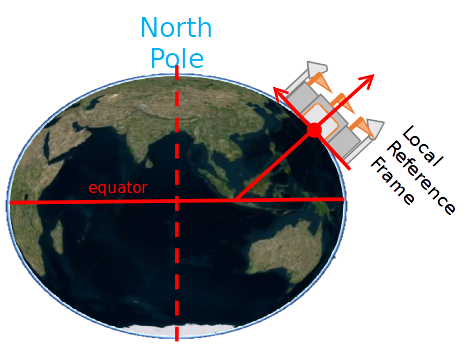
\includegraphics[width=0.6\linewidth]{local-ref-frame.png}
  \caption{Example of setting up a local reference frame. World coordinates are converted to vectors relative to the Cartesian coordinate system centred at the stadium in the figure. Note that the up axis does not exactly intersect the centroid of Earth---this is due to a subtlety in the definition of geodetic latitude of an ellipsoid Earth to be tangent to the ellipsoid (which is also the approximate direction of gravity, ignoring localised Deflection Of Vertical) rather than radiated from the centroid.}
  \label{fig:local-ref-frame}
\end{figure}

It is first necessary to convert geodetic latitude and longitude angles into
three-dimensional Cartesian space. The equations to convert a WGS84 location
represented as longitude \(\lambda\), latitude \(\phi\), and height
\(h\) to Earth Centred Earth Fixed (ECEF) x,~y,~z coordinates relative to
the centre of Earth are taken from \cite{drake_converting_2002} and presented in Eq.~\ref{eq:ecef}.

% 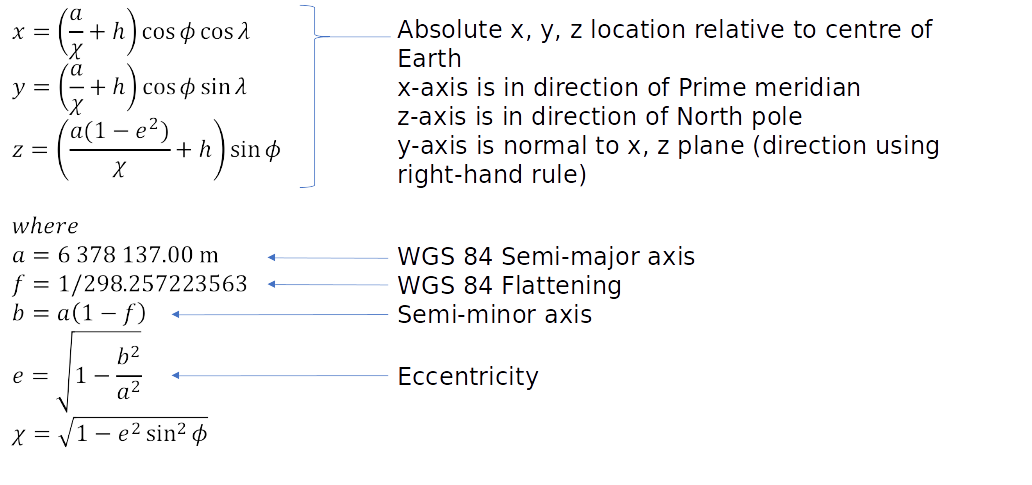
\includegraphics[width=1.0\textwidth]{matrix-formulas-1.png}
% Converted from Word (matrix-formulas-1.png)
\begin{minipage}{\linewidth}
\begin{align} \label{eq:ecef}
\left.\begin{aligned}
      x &= \left(\frac{a}{\chi}+h\right)\cos{\phi}\cos{\lambda} \\
      y &= \left(\frac{a}{\chi}+h\right)\cos{\phi}\sin{\lambda} \\
      z &= \left(\frac{a(1-e^2)}{\chi}+h\right)\sin{\phi} \\
      \end{aligned}
\right\}
\qquad
\begin{aligned}
& \text{Absolute x, y, z location} \\
& \text{relative to centre of Earth.}
\end{aligned}
\end{align}
where
\begin{description}
\item[$x$] is in the direction of the Prime meridian.
\item[$z$] is in the direction of the North pole.
\item[$y$] is in the direction normal to the x, z plane\newline(using right-hand rule).
\item[$e = \sqrt{1-\frac{b^2}{a^2}}$] is the eccentricity.
\item[$a = 6\ 378\ 137\ \mathrm{\mathrm{m}}$] is the WGS 84 semi-major axis.
\item[$b = a\left(1-f\right)$] is the WGS 84 semi-minor axis.
\item[$f = 1/298.257223563$] is the WGS 84 flattening.
\item[$\chi = \sqrt{1-e^2\sin^2{\phi}}$]
\end{description}
\end{minipage}

The equations to convert a WGS84 point (x,~y,~z) from ECEF coordinates
into local East North Up (ENU) coordinates (de,~dn,~du) with respect to
a local fixed reference frame at \(\lambda_{ref}\), \(\phi_{ref}\),
\(h_{ref}\) are taken from \cite{drake_converting_2002} and presented in Eq.~\ref{eq:matrix}.

%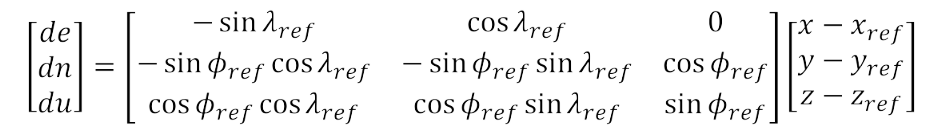
\includegraphics[width=0.7\textwidth]{matrix-formulas-2.png}
% Converted from Word (matrix-formulas-2.png)
\begin{equation} \label{eq:matrix}
\left[
\begin{matrix}
de\\
dn\\
du\\
\end{matrix}
\right]=\left[
\begin{matrix}
-\sin{\lambda_{ref}}&\cos{\lambda_{ref}}&0\\
-\sin{\phi_{ref}}\cos{\lambda_{ref}}&-\sin{\phi_{ref}}\sin{\lambda_{ref}}&\cos{\phi_{ref}}\\
\cos{\phi_{ref}\cos{\lambda_{ref}}}&\cos{\phi_{ref}\sin{\lambda_{ref}}}&\sin{\phi_{ref}}\\
\end{matrix}
\right]
\left[
\begin{matrix}
x-x_{ref}\\
y-y_{ref}\\
z-z_{ref}\\
\end{matrix}
\right]
\end{equation}


where \(x_{ref}\), \(y_{ref}\), \(z_{ref}\) are the x,~y,~z coordinates of
the origin of the reference frame calculated using Eq.~\ref{eq:ecef}.

The above formulas do not include a term to correct for azimuth,
\(\alpha_{ref}\), in the case of a rotated reference frame. However,
this can easily be included by pre-multiplying by yet another rotation
matrix to rotate about the up axis.

\subsection{Projecting Geographic Coordinates to a Local
Projection}\label{projecting-geographic-coordinates-to-a-local-projection}

Map makers have devised two-dimensional projections of the Earth that can preserve
distance to a point, angles, or area, but it is impossible to have all
three at the same time. While computerised maps can use three-dimensional coordinates to perform exact geodesic calculations over the curvature of Earth,
these are computationally intensive, and furthermore, they limit spatial
analysis techniques to those for which a geodesic algorithm is
available. For mapping within a small region, calculations can be approximated within the two-dimensional projection,
but appropriate projection parameters must be chosen for that region. Note
that unlike local reference frames described in the previous section,
cartographic projections are designed to preserve properties along the
curvature of Earth, so are appropriate for much larger regions (although
for projections of the entire Earth, severe distortion is still
inevitable).

In his classic work, \emph{Map projections: A working manual}
\cite{snyder_map_1987}, John P. Snyder sets out guidelines for
selecting the appropriate map projection given the location and scale of
the map needed. For brevity, this section will focus on Hotine's
Oblique Mercator projection, a conformal (angle preserving) projection
suitable for mapping small rectangular regions, narrow with respect to
the curvature of Earth.

Hotine's Oblique Mercator (also known as Rectified Skew Orthomorphic)
attempts to preserve scale along a central line chosen by the map maker.
Hotine's Oblique Mercator is also conformal (no local angular
distortion) away from central line. To achieve this, Hotine's Oblique
Mercator projection must compromise by distorting area away from the
central line. Note that while the projection preserves local angles
(i.e.~relative angles within any infinitesimal portion of the map),
global angles (such as azimuth) are still distorted.

Hotine's Oblique Mercator projection can be parameterised to the region
of interest. Much like the information required to set up a local
reference frame in the previous section, the information needed to
parameterise Hotine's Oblique Mercator projection is a reference
location, and a reference angle. \figref{fig:omerc-proj} provides
an example of Hotine's Oblique Mercator centred around Melbourne, in an
eastward direction towards the lower half of the US. This projection
would be ideal for tracking the ground path of a flight from Melbourne
to the US.

\begin{figure}[htbp]
  \centering
  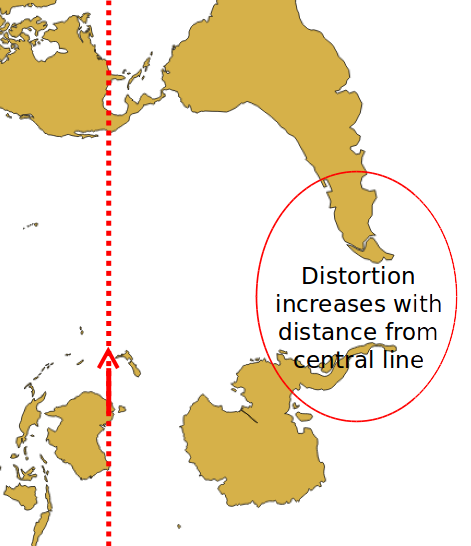
\includegraphics[width=0.5\linewidth]{omerc-proj.png}
  \caption{Example of Hotine's Oblique Mercator projection taken at Melbourne in east direction. Note the severe distortion in the tail of Antarctica and South America in this projection, due to their distance from the choice of central line.}
  \label{fig:omerc-proj}
\end{figure}

Whilst local projections are conceptually different to reference frames,
the similar information required to build a Hotine's
Oblique Mercator projection (and its alternatives) versus a local
reference frame, allows projections to serve as a natural extension of
Reference Frames when concerns shift from studying very small
(i.e.~approximately uniform direction of gravity) regions of the Earth
towards larger regions where the analyst is interested in the positions
of objects relative to the curvature of the Earth (i.e.~a non-Euclidean
coordinate space).

The formulas for a computerised implementation of Hotine's Oblique
Mercator projection can be found in Hooijberg \cite{Hooijberg2008} and Evenden \cite{evenden_libproj4_2005}. In modern times, cartographers are
unlikely to ever need to ever implement projection computations
themselves, as computations are tedious, and can be error prone if not
implemented carefully and tested thoroughly. Instead, cartographers
would use a readily available implementation, such as that found in the
Open Source PROJ.4 \cite{evenden_libproj4_2005} library.

% \textbf{Todo:} Concepts one must know, steps, complexity of task. Show
% on a plot (Measure approximate number of steps. Can ignore units for
% complexity).

\subsection{Support for Coordinate Transformations within Geographic
Information
Systems}\label{support-for-coordinate-transformations-within-geographic-information-systems}

Geographic Information Systems (GIS), such as QGIS\footnote{{[}Software{]}
  QGIS Project, ``QGIS: A Free and Open Source Geographic Information
  System''. \url{http://www.qgis.org/} Accessed: 2017-03-16}, provide the user
with a graphical user interface to convert data between different
coordinate systems. Typically, datasets will be encoded in a
standardised coordinate reference system, such as one of the reference
systems encoded in the ESPG database\footnote{International Association
  of Oil \& Gas Producers, ``ESPG Geodetic Parameter Dataset''.
  \url{http://www.epsg.org/} Accessed: 2017-03-16}. Metadata describing the
projection format is usually stored alongside the dataset, and the
interface to convert to a different standardised coordinate system is
usually as simple as selecting ``save as\ldots{}'', then selecting the
name of the coordinate system from a list. This not only hides the
complexity of performing the transformation from the user, it also hides
the need for a user to understand how coordinate systems are
represented, so long as the user knows the identifier for the coordinate
reference system they wish to work in. The Universal Transverse Mercator
system can be used to generate a set of coordinate reference systems by
splitting the Earth's ellipsoid into narrow strips of 6 degrees longitude in
which distortion is minimal. For example, an appropriate projection for
planning a railway between Melbourne and Cairns (north bound of
Melbourne) would be Map Grid Australia 55 (UTM zone 55 of the GRS80
ellipsoid\footnote{spatialreference.org, ``EPSG:28355 (GDA94 / MGA zone
  55)''. \url{http://spatialreference.org/ref/epsg/28355/} Accessed:
  2017-03-16}, officially defined as using the Geocentric Datum of
Australia\footnote{Geoscience Australia, ``Geocentric Datum of Australia
  (GDA)''.
  \url{https://web.archive.org/web/20170218103859/http://www.ga.gov.au/scientific-topics/positioning-navigation/geodesy/geodetic-datums/gda}
  Accessed: 2017-03-16}) thus avoiding the need for the user to define
their own coordinate system.

However, in the case of creating a coordinate reference system with respect to
some object, it is necessary for the user to define their own coordinate
reference system. If the user's sole objective is simply to make the
reference object (0,0) for convenience, then this can be achieved by
using an existing coordinate reference system and adding a so-called
``false-easting'' and ``false-northing'' to linearly offset coordinates
by some fixed amount. However, shifting the coordinate system in this
manner does nothing to address the distortion properties of the
projection. For example, it is incorrect to use false-easting and
false-northing to shift an existing coordinate reference system to some
other part of the globe, as its only effect is to make the numbers more
convenient---one would still be working in an area with extreme
distortion. Some GIS tools include an affine transformation tool to
shift object coordinates, but similarly to the false-easting and
false-northing approach, this also does nothing to address distortions
due to the curvature of Earth when objects are shifted large distances.
In order to create a projection with minimal distortion about a
reference point, it is necessary to set the parameters of the projection such
that the projection is calculated about that reference point.

Unfortunately, defining a custom coordinate reference system using existing GIS
software is often a cumbersome process. In QGIS, a user must manually
write a projection string, using a specification format such as
Well-Known Text (WKT) or PROJ.4. An example is provided in Listing
\ref{lst:proj}\footnote{The PROJ.4 template for setting up a Hotine's
  Oblique Mercator (omerc) projection relative to a reference point and
  reference angle comes from AndreJ's answer to ``Using customized
  Coordinate System in ArcGIS Desktop?'' on the Geographic Information
  Systems Stack Exchange
  \url{http://gis.stackexchange.com/questions/83861/using-customized-coordinate-system-for-archaeological-site-data/83884\#83884}
  Accessed: 2017-02-03}. Given that GIS tools dedicate a large area of
the screen to an interactive map for selecting points, it is surprising
that users must manually type or copy-paste the coordinates to define
the centre-point of the coordinate reference system. Furthermore, unless working with
a projection that preserves azimuth angles (such as the Mercator
Projection), care must be taken to ensure that the azimuth is measured
with respect to north, rather than the vertical direction in the current
map projection, which may be distorted.

% Supervisor: {Articulate ``cumbersome'' as
%   a combination of: steps, complexity. If these are not done regularly,
%   then people forget and hence frequency of task also matters. Would be
%   good to have a table that identifes these as an illustration of
%   ``cumbersome'', ``tedious''}

\begin{lstlisting}[frame=single,caption=Above: Example of a PROJ.4 expression for a Hotine's Oblique Mercator projection centred at the Melbourne Cricket Ground in the direction of the goal posts at N86\textdegree E.,label=lst:proj]
+proj=omerc
+lat_0=-37.8200
+lonc=144.9835
+alpha=86
+k=1
+x_0=0
+y_0=0
+gamma=0
+ellps=WGS84
+towgs84=0,0,0,0,0,0,0
+units=m +no_defs
\end{lstlisting}

\begin{figure}[htbp]
\centering
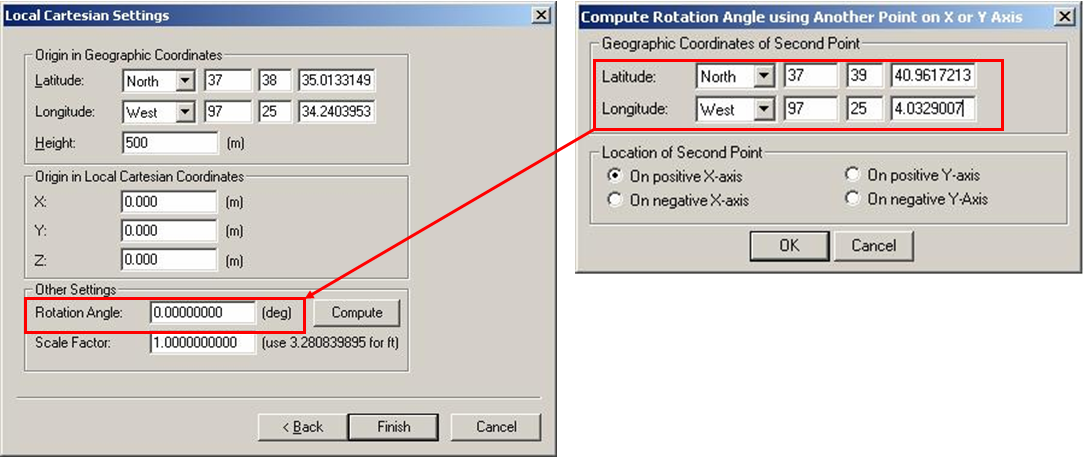
\includegraphics[width=0.8\linewidth]{figs/spatial/novatel.png}
\caption{NovAtel GrafNav provides an interface to convert GPS data in world coordinates to a local coordinate system. However, configuring the local coordinate system requires manually specifying coordinates. Screenshots \copyright{}~NovAtel~Inc. taken from software documentation. %), which can be tedious when there are multiple involved (e.g. teams that play on different fields).
\label{fig:novatel}}
\end{figure}

NovAtel GrafNav\footnote{NovAtel, ``Creating a Local Cartesian Plane,''
  Waypoint FAQs. \url{http://www.novatel.com/products/software/waypoint-faqs/}
  Accessed: 2017-03-16} provides a streamlined interface for creating
local coordinate systems, shown in \figref{fig:novatel}. The interface only requires the essential
information from the user: reference latitude, reference longitude,
reference height, and reference rotation angle. Alternatively, the
interface can infer the rotation angle of the reference system if the
user provides a second point along an axis. Once the reference system
has been established, the user is free to bulk-reproject data points to
their reference system. The system only provides the option to
project to Cartesian coordinates in a local reference frame, and does
not appear to offer the ability to use the reference system as a basis
for a cartographic projection. Similarly to the issues described relating to the user interface for defining reference frames in GIS software, the
interface appears to require the user to manually enter the coordinates,
thus would be tedious if the user wished to set up multiple local
reference frames.

\begin{figure}[htbp]
\centering
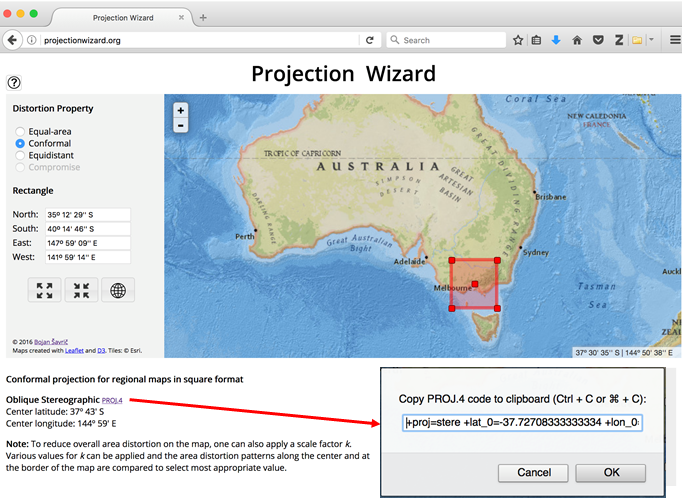
\includegraphics[width=0.8\linewidth]{figs/spatial/proj-wizard.png}
\caption{Projection Wizard \cite{savric_projection_2016} allows the user to visually draw a rectangle, and will automatically generate an appropriate PROJ.4 projection string for that area. However, it is not possible for the user to draw a rotated region, thus support for generating oblique projections is limited.
\label{fig:proj-wizard}}
\end{figure}

Projection Wizard \cite{savric_projection_2016} implements the
guidelines by John P. Snyder \cite{snyder_map_1987} to automatically
suggest the most appropriate projection based upon a bounding box drawn
by the user on an interactive map of the Earth (see \figref{fig:proj-wizard}). Unfortunately, it doesn't
currently allow the user to draw an oblique (rotated) bounding box, thus
is limited to projections where north is at the top of the map. While
Projection Wizard doesn't implement any functionality to reproject data
automatically, it can generate a PROJ.4 projection string. The user
could then copy-paste this projection string into their GIS tool to
define a coordinate reference system, or use it to bulk reproject data
using the PROJ.4 Unix command line tool.

% \textbf{TODO:} Need a summary of key problems \emph{here} and with show
% this with a few paragraphs is all that may be needed in the
% \emph{paper}. The current content is needed for the \emph{thesis} So
% leave it.

\begin{figure}[htbp]
\centering
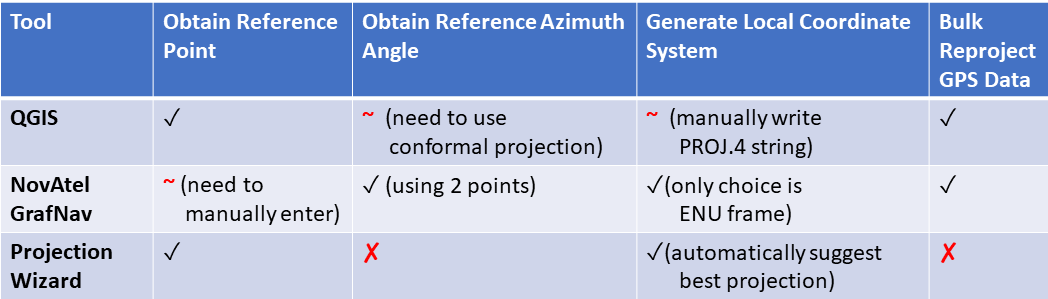
\includegraphics[width=\linewidth]{figs/spatial/tool-comparison-table.png}
\caption{Comparison of geospatial systems that provide ability to convert GPS world coordinates to local coordinates.\\Key: \cmark=supported, \xmark=not~supported, $\sim$=partial~support.%\textbf{TODO:} Convert from MS Powerpoint (screenshot) to Latex. %Nope.
\label{fig:tool-comparison-table}}
\end{figure}

A comparison of systems discussed in this section for converting GPS trajectory data to local coordinates (e.g. local x-y coordinates of the relevant sport field) is provided in \figref{fig:tool-comparison-table}. While systems (or combinations of systems) exist to perform the conversion, none offer an streamlined end-to-end process for performing the conversion in a manner that is suited to non-expert users (e.g. sport performance analysts as opposed to professional GIS analysts).

%\subsection{Support in existing sport player tracking systems}
\subsection{Support for Coordinate Transformations within Sport Player Tracking Software}

\begin{figure}[htbp]
\centering
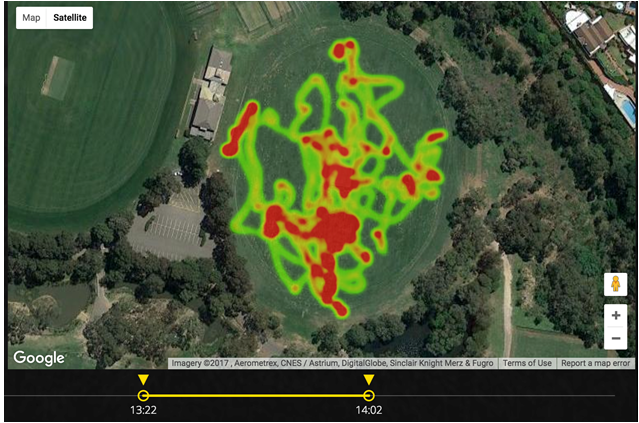
\includegraphics[width=0.8\linewidth]{figs/spatial/spt-gametraka.png}
\caption[SPT GameTraka]{SPT GameTraka\protect\footnotemark{} is capable of generating a heat-map of player location overlaid on Google Maps.
\label{fig:spt-gametraka}}
\end{figure}
\footnotetext{\url{http://demo.gametraka.com} Accessed: 2017}

% http://www.catapultsports.com/au/media/catapult-sports-is-google-analytics-for-athletes-wearable-technology-start-up-series/
% https://www.slideshare.net/MatGlasson/2015ssaescansfr
% -> Nate Cochrane, 19th June 2014, ‘Catapult Sports is ‘Google analytics for athletes’: wearable technology start- up series’, BRW, http://www.brw.com.au/
% http://pandora.nla.gov.au/tep/12279 Pandora archives are restricted for 70 years.

% Support for spatial analysis of teams provided by existing GPS player tracking software appears limited.
% To better understand these issues, state-of-the-art in sport, commercial systems were examined.

The previous sections motivated the need to transform data to a local coordinate system, highlighted the theoretical issues surrounding performing this conversion correctly, and showed that general purpose systems for performing this conversion are not well suited for non-expert users and are tedious when conversions to many different local systems are necessary (i.e. pairing GPS trajectories over the course of the season with the relevant sport field). For completeness, a selection of commercial software systems for analysing sport player position tracking data were examined.

\textit{SPT GameTraka} (\figref{fig:spt-gametraka}) generates a heat-map of player location overlaid on Google Maps. Firstly, note that all maps are north oriented, which makes it difficult to compare patterns on a field that is N-S oriented to a field that is E-W oriented. Further note that the software has no internal model of the field, thus it is not possible to quantitatively break down data by zone of field. Instead SPT GameTraka focuses on statistics such as distance, speed, intensity, etc. that can be computed without reference to the field.

\textit{GPSports Team AMS} (\figref{fig:limitations-of-gpsports-team-ams}) converts GPS data to x-y coordinates to allow quantitative analysis of position. However, the origin and orientation of the x-y coordinate system appear to be arbitrary, thus it is difficult to compare x-y values between different fields.

\begin{figure}[H]
\centering
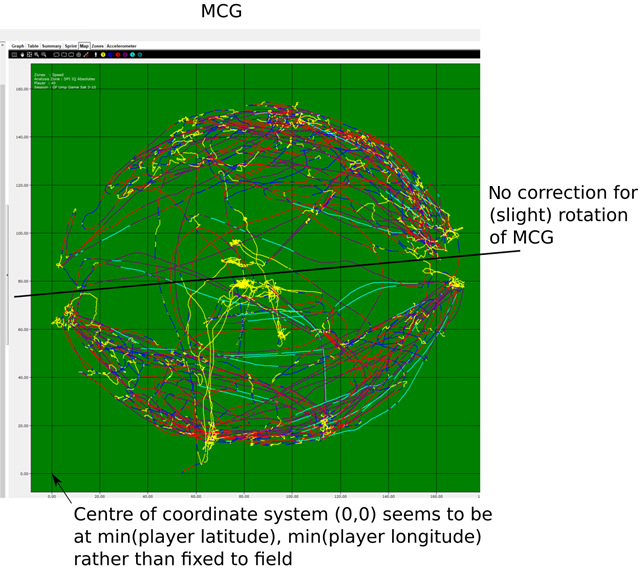
\includegraphics[width=0.75\linewidth]{figs/spatial/limitations-of-gpsports-team-ams.png}
\caption{Analysis of GPS tracking data using Team AMS (software provided with GPSports GPS tracking devices). Note arbitrary origin and orientation of x-y coordinate system. This makes spatial comparisons of tracking data from different venues challenging.
\label{fig:limitations-of-gpsports-team-ams}}
\end{figure}

The software provided with the \textit{Catapult Sports ClearSky} local positioning system works in x-y positions relative to the playing field (\figref{fig:catapault-sports}). Due to the limited publicly available documentation, it is unclear whether their software provides a way to perform similar analysis using GPS tracking devices as opposed to local positioning devices.\footnote{One retailer of Catapult Sports OptimEye GPS tracking devices states they provide the ability to ``build your own field with the OptimEye units''; however, it is unclear what this entails. \url{http://performbetter.co.uk/product/catapult-optimeye-x4-athlete-monitoring-system/}. Accessed \dt{2019-06-08}}

% This is trivial,
% (\figref{fig:limitations-of-gpsports-team-ams}) converts GPS data to x-y coordinates to allow quantitative analysis of position (\figref{fig:limitations-of-gpsports-team-ams}). These the origin and orientation of the x-y coordinate system appear to be arbitrary, thus there is difficult to compare x-y values between different fields.


\begin{figure}[htb]
\centering
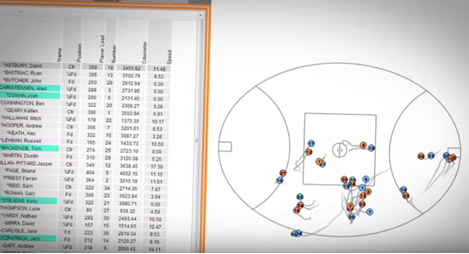
\includegraphics[width=0.9\linewidth]{figs/spatial/catapault-sports.png}
\caption[Catapult Sports ClearSky local positioning system]{Catapult Sports ClearSky local positioning system (from promotional video\protect\footnotemark{}). Local positioning systems use beacons placed around the field to capture player positions in x-y form. However the system is many times more expensive than GPS tracking devices, and in the past Catapult Sports have charged \$100,000 per year per club.\protect\footnotemark{} 
\label{fig:catapault-sports}}
\end{figure}
\addtocounter{footnote}{-1}
\footnotetext{[Video] Catapult Sports, 2013, ``Catapult ClearSky.'' \url{https://youtu.be/lVKgPk1S7L0?t=1m41s}}
\addtocounter{footnote}{1}
\footnotetext{``Catapult Sports is `Google analytics for athletes': wearable technology start-up series'' \url{https://web.archive.org/web/20160901160002/http://www.catapultsports.com/media/catapult-sports-is-google-analytics-for-athletes-wearable-technology-start-up-series/}}

\pagebreak{}

As highlighted, converting GPS tracking data to the local coordinate system of the field is a necessary pre-requisite for comparing GPS tracking data across different fields. However, this functionality appears to be poorly supported by existing software, other than by software provided with local positioning systems which require physical beacons placed around the field. Types of sport that involve travelling large distances where it is necessary to account for the curvature of Earth, e.g. long distance boat races, are most at risk if the geospatial transformations are not properly understood. %However, the limited documentation surrounding sport software suggests problem.

% \nb{It was interesting that at the (unrecorded) Victoria University Player Tracking Workshop (VUPTW) run by Alice Sweeting and Sam Robertson on 13 Feb 2019, David Corbett (PhD candidate, Victoria University), presented on solving exactly the same issue of converting longitude,~latitude to x,~y coordinates of the field in order to progress with his own PhD. When I discussed with him, he said he intends to release this as an open source R package after his PhD, but has not yet formally published anything about it. May be worth arranging to cite each other's solutions (once released) to make it easier for anyone encountering this problem in future to reuse existing work rather than starting from scratch.}
